%!TEX root = ../report.tex

\chapter{Methodology}
\label{chapter:methodology}
This chapter concentrates on the methodology incorporated to automatically configure the coupling tool of a multiphysics simulation with optimal parameters. The study focuses on Fluid-Structure Interaction (FSI), transient study multiphysics simulations. The chapter begins with the motivation for using Automated Algorithm Configuration (AAC) in the approach, an overview of the proposed solution, followed by an extensive description of the various components of AAC. In addition, the chapter encompasses a brief description of Bayesian optimization and a flowchart of Sequential Model-based Algorithm Configuration (SMAC).
    
\section{Proposed strategy}

The research work aims to automatically configure the coupling tool, MpCCI, with optimal parameters to reduce the run-time of the simulation. The process of configuring the coupling tool is an online prediction of optimal configuration for a particular simulation feature set provided by the user. The intuition is employing a machine learning model to predict the optimal configurations. To train the model (offline task) and predict the optimal configuration for a given feature set, the knowledge of the best configuration of feature set is imperative. The optimal configurations for a particular feature set are identified by black-box optimization of each feature set. The types of parameters involved in the black-box optimization task are categorical, numerical, and conditional parameters. In addition, a forbidden set of parameter combinations are available. The problem of optimizing a black-box function with various types of parameters is the reason for employing SMAC, an AAC procedure. The complete system configuring the parameters of the coupling tool with optimal values is an AAC procedure. This formulates the research work under the branch of AAC.

The proposed solution is the pipeline illustrated in figure \ref{fig:processflow} for configuring the coupling tool with the optimal parameter configuration with relatively lesser run-time than the current default configurations used for simulations. The pipeline is divided into two parts- offline and online. The offline part is the development phase starting from developing simulation problems to generate dataset followed by training machine learning models. The online part depicts the idea of the smart coupling tool. The smart coupling tool incorporates the machine learning models trained during the offline development phase to suggest the optimal parameter configuration to the user provided simulation problem.

\begin{figure}[!ht]
\centering
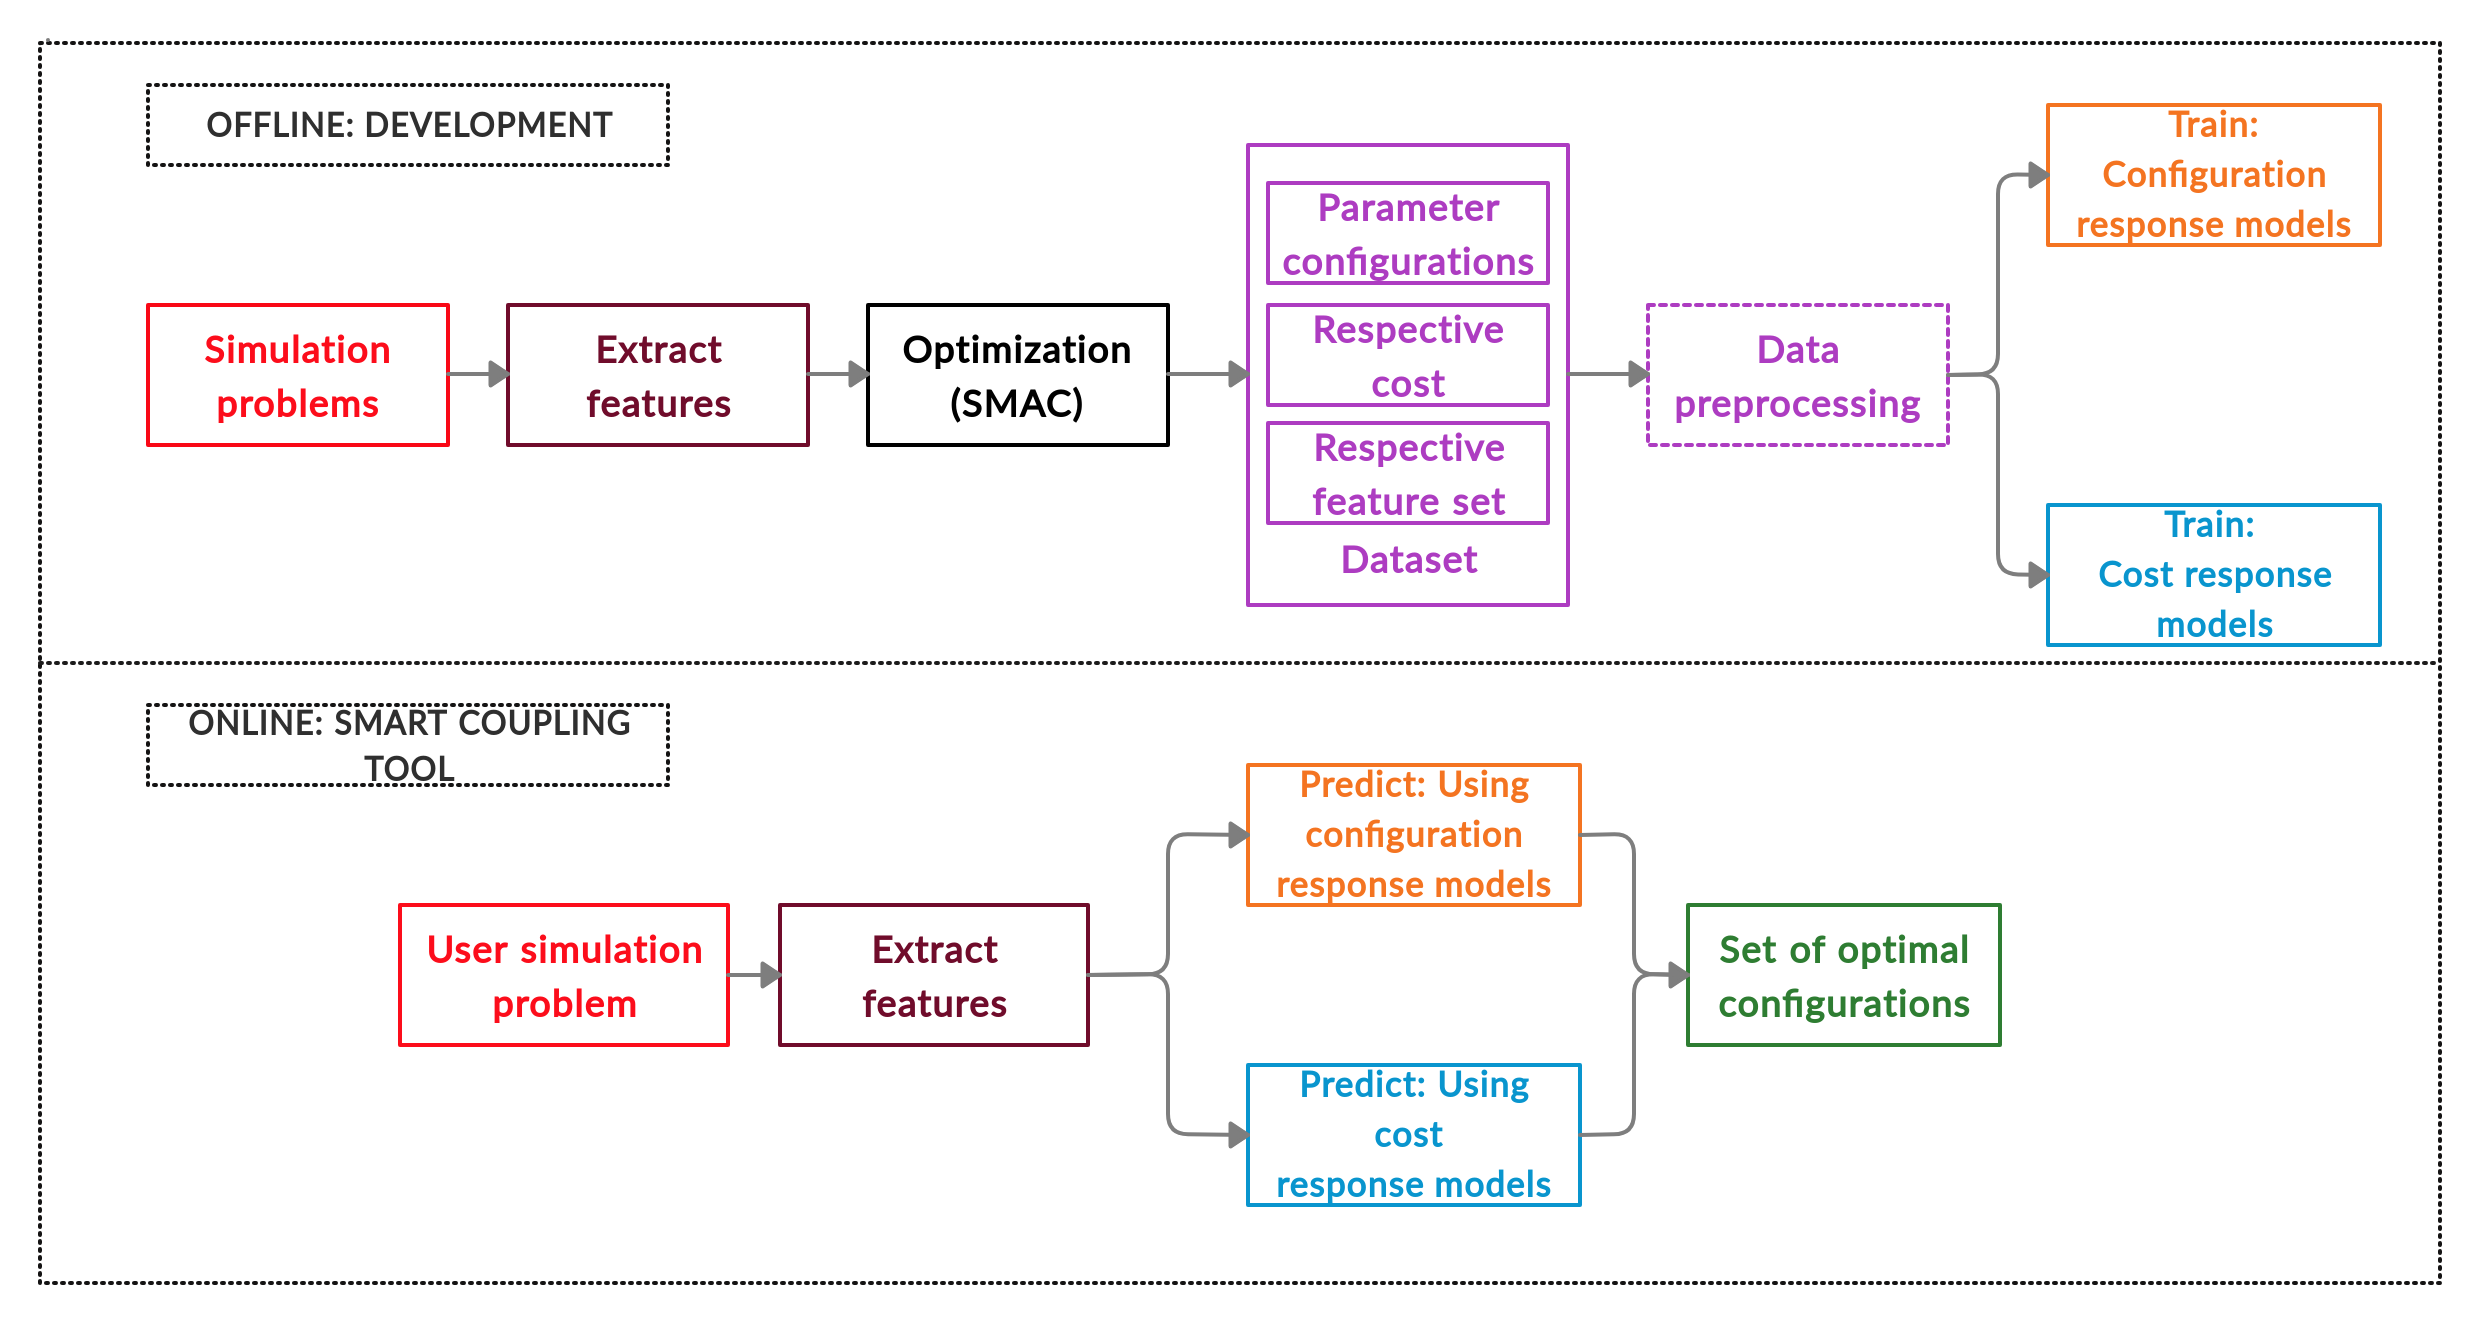
\includegraphics[width=1\linewidth,height=0.43\textheight]{images/Processflow.jpg}
\captionsetup{justification=justified}
\caption[Overview of the proposed strategy to predict optimal parameter configuration]{Overview of the proposed strategy to predict optimal configuration. Two parts of the pipeline- development and smart coupling tool. The inputs (red) are the FSI simulation problem to the respective parts of the pipeline. The extract features block (brown) extracts the features of the simulation instances. The dataset (purple) is the multiphysics simulation data set generated by single simulation instance optimization. The optimization is performed by SMAC (black). The data pre-processing stage (dashed purple) performs data cleaning and normalization for the training process. Two types of models- configuration response (orange), cost response (blue) are trained. Finally, a set of desirable optimal configurations (green) are predicted. The color resemblances between the online and offline parts of the pipeline illustrate the usage of the same machine learning model, similar feature extraction method and similar simulation problem type.}
\label{fig:processflow}
\end{figure}

Firstly, a set of simulation instances across different simulation problems with a different feature set spanning the domain of multiphysics simulation is selected. Owing to the time constraint and primary need to test the research hypothesis (applicability of AAC approach for automatically configuring the coupling tool), the number of simulation problems is restricted to two. 
    
Secondly, a set of features representing the simulation instance has been extracted using the feature reader module \ref{section:feature_reader}. The features are used to enrich the RF surrogate model of SMAC. A surrogate model approximately mimics the behaviour of the coupling tool using the data collected on evaluating the simulation instances with different configuration settings. The features aid the model in learning about the instance. However, SMAC optimizes the simulation instance by performing the actual simulation with different valid parameter configurations. Therefore, the output of SMAC is different parameter configurations SMAC evaluated on the instances with the respective cost and the respective feature set of the simulation instance. This set of outputs from SMAC serves as the dataset from the next phase of training machine learning models.
    
The models has been trained in two different approaches- Configuration response and Cost response models to predict the optimal configurations. In the online prediction phase, the trained models are used for inference.  The online prediction will be integrated to the coupling tool in future. In this research project, the complete pipeline- optimization phase, training phase and prediction phase has been completed.
    
%     The methodology can be decomposed into 4 phases namely- Optimization, Normalization, Training and Prediction. The section \ref{section:optimization} provides an illustrative explanation of Bayesian optimization followed by an extended flowchart of Sequential Model-based Algorithm Configuration (SMAC). The section \ref{section:trainingphase} and \ref{section:predictionphase} portrays the methodology adapted to train and predict the optimal parameters of the coupling tool given a problem instance by the user respectively.
    
\section{Hyperparameters of the coupling tool}
 \label{section:hyperparameters_couplingtool}  
The coupling tool, MpCCI performs a multiphysics simulations by solving the governing equations of the physical domain. Therefore, the entire problem is viewed to be solving system of equations. The governing equations concerning the solid domain are solved by the structural solvers (structural code) such as Abaqus, ANSYS, Calculix, and Marc. The fluid domain governing equations are solved by fluid solvers (fluid code) such as OpenFOAM, FineOpen and ANSYS FLUENT. The fluid flow is described by the Navier-Stokes equations given in \cite{FSICartesiangrid}. Similarly, the solid mechanics is described by the stress, strain tensors, and Hooke’s law given in \cite{FSICartesiangrid}. The equations are iteratively solved. In a transient problem, a single time step includes several iterations until a particular time step converges for both solvers.

The hyperparameters of the coupling tools performing FSI transient study simulations are coupling scheme, initial exchange, relaxation\_0, relaxation\_1, relaxation method, relaxation factor, Andersonmix type, number of levels, omega, ramp\_0 and ramp\_d. The parameters of the coupling tool largely impact the accuracy, stability and run-time of the simulations. This section provides a description of the hyperparameters configured in this research work.

\subsection{Coupling scheme}

There are two coupling schemes available for co-simulation, namely, explicit and implicit. Explicit (loose or weak) coupling involves the computation of the solution directly from the quantities known. At a particular time step, the solid and fluid code exchanges information once in explicit coupling. 
% https://core.ac.uk/download/pdf/11679615.pdf
To preserve the equilibrium between the solid and fluid solvers at every time step and obtain precise results, implicit coupling is used. Implicit coupling includes solving a system of coupled equation in an iterative procedure. Each time step of the solvers is carried out until convergence or maximum iterations. The data exchange between the solvers occur at each iteration of the time step \cite{couplingscheme}.

\subsection{Initial exchange}

The parameter initial exchange in MpCCI determines the coupling algorithm and the data exchange pattern between codes. The possible initial exchange settings are:

% The two types of coupling algorithms for bidirectional communication are serial and parallel coupling.
% In transient study, the codes of each solvers are initialized to transfer data in two scenarios, namely, at the beginning or at the end of each time step and before or after a particular iteration step of a time step. 
% The three actions of the solver codes concerning data exchange are receive, send, and exchange. The receiver code waits for data always. In contrast, the sender code never waits for data. The exchange involves a send and receive without any order. 

\begin{itemize}

\item receive:exchange - The simulation code A and B in figure \ref{Fig:receiveexchange} is initialized to perform receive and exchange actions, respectively. The code A receive data from the partner code B, shown by encircled 1 (step 1). Once it receives data from B, A performs computation in step 2. The exchange action comprise send and/or receive action. The code B sends data at step 1 and receives data at step 3 after A completes the computation. The code B performs computation in step 4 once it receive the data from A. Finally, step 5 is similar to step 1. This coupling algorithm is serial coupling as illustrated in figure \ref{Fig:receiveexchange}.

\begin{figure}[!ht]
\centering
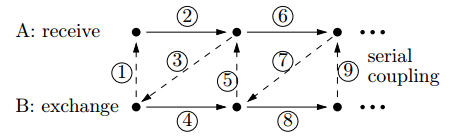
\includegraphics[width=\textwidth]{images/IE1.png}
\captionsetup{justification=justified}
\caption[Initial exchange setting- receive:exchange]{Initial exchange setting- receive:exchange \cite{MpCCI_documentation}.}
\label{Fig:receiveexchange}
\end{figure}

\item exchange:receive - This setting is used in serial coupling algorithm. The simulation code A and B is initialized to perform exchange and receive actions, respectively.

\item exchange:exchange - It is used in parallel coupling. The simulation code A and B in figure \ref{Fig:exchangeexchange} is initialized to perform exchange action. At step 1, A and B exchange data simultaneously. Then in step 2, A and B performs computations in a parallel manner followed by simultaneous data exchange (step 3).

\begin{figure}[!ht]
\centering
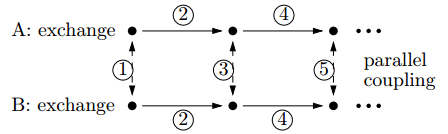
\includegraphics[width=\textwidth]{images/IE2.png}
\captionsetup{justification=justified}
\caption[Initial exchange setting- exchange:exchange]{Initial exchange setting- exchange:exchange \cite{MpCCI_documentation}.}
\label{Fig:exchangeexchange}
\end{figure}

\end{itemize}

\subsection{Relaxation method}

Relaxation method is an iterative procedure for solving system of sparse linear equations and non-linear equations \cite{relaxationmethod_intro}. The sparse linear system of equations are obtained from the discretizations of differential equations by finite-differencing. Relaxation methods are used in multiphysics simulations to stabilize and increase the convergence speed of a non-linear coupled process. The 4 relaxation methods available in MpCCI are:

\begin{itemize}
    \item Fixed
    \item Ramping
    \item Aitken
    \item Quasi-Newton
\end{itemize}

Anderson mixing, ramp\_0, ramp\_d, and omega are various child parameters associated with different relaxation methods. A detailed explanation on the relaxation methods is provided in \cite{MpCCI_documentation}. 

% In coupled processes, a quantity is modified to achieve stable results for a time step before passing the quantity to the simulation code of the partnering coupled domain. The iterative relaxation method checks for a relaxation tolerance for each time step of the coupling process. At a particular iteration k, the relaxation occurs in a manner the quantity $Q^k$ and $Q^k_{\text{relaxed}}$ are approaching each other at a particular coupling step. The coupled system reaches equilibrium resulting a solution at $Q^k$ $\approx$ $Q^k_{\text{relaxed}}$ \cite{MpCCI_documentation}.

% The 4 relaxation methods available in MpCCI are discussed in the following subsections. The equations in the below sections are adapted from the MpCCI manual \cite{MpCCI_documentation}.

% \subsubsection{Fixed relaxation} The relationship between the relaxed quantity in the next iteration, $Q^{k+1}_{\text{relaxed}}$ and the true quantity $Q^{k+1}$ is given by the following equation \ref{equation:fixed} \cite{MpCCI_documentation}.

% \begin{equation}
% Q_{\mathrm{relaxed}}^{k+1}=\alpha \cdot Q^{k+1}+(1-\alpha) \cdot Q_{\mathrm{relaxed}}^{k}
% \label{equation:fixed}
% \end{equation}

% In the equation \ref{equation:fixed}, $\alpha$ is the relaxation factor. It is one of the hyperparameters of this research study. $Q^k_{\text{relaxed}}$ is the relaxed quantity at iteration k. The relaxed quantity is transferred to the receiver simulation code. $\alpha$ $<$ 1 is under-relaxation and $\alpha$ $>$ 1 is over-relaxation. $\alpha$ is selected by the user depending on the problem at hand.

% \subsubsection{Ramping} This is a relaxation method involving a linearly increasing or decreasing behavior of the relaxation factor until a convergence of the consecutive relaxed values. The receiver receives a relaxed quantity given by the equation \ref{equation:ramping} \cite{MpCCI_documentation}.

% \begin{equation}
% \begin{aligned} Q_{\text {relaxed }}^{k+1} &=\beta^{k} \cdot Q^{k+1}+\left(1-\beta^{k}\right) \cdot Q_{\text {relaxed }}^{k} \\ &=Q_{\text {relaxed }}^{k}+\beta^{k} \cdot\left(Q^{k+1}-Q_{\text {relaxed }}^{k}\right) \end{aligned}
% \label{equation:ramping}
% \end{equation}

% The factor $\beta^k$ denotes the ramping factor at iteration k+1 of the relaxation method. $\beta^k$ is given by the equation \ref{equation:beta} \cite{MpCCI_documentation}.

% \begin{equation}
% \begin{array}{ll}{\beta^{k}=\min \left(1, \beta_{0}+(k+1) \cdot \beta_{d}\right)} & {\text { for under-relaxation ramping }} \\ {\beta^{k}=\max \left(1, \beta_{0}-(k+1) \cdot \beta_{d}\right)} & {\text { for over-relaxation ramping }}\end{array}
% \label{equation:beta}
% \end{equation}

% $\beta_0$ and $\beta_d$ are the initial and step value of ramping referred by initial ramp value and ramp delta.  The values $\beta_0$ and $\beta_d$ are also parameters of the coupling tool.

% \subsubsection{Aitken} The Aitken relaxation method computes the relaxation factor in an adaptive manner depending on the previous iteration values of the relaxed and actual quantities sent to the receiver code. The relaxed quantity sent to the receiver at iteration k+1 is given by the following equation \ref{equation:Aitken} \cite{MpCCI_documentation}.

% \begin{equation}
% Q_{\mathrm{relax}}^{k+1}=\omega^{k} \cdot Q^{k+1}+\left(1-\omega^{k}\right) \cdot Q_{\mathrm{relax}}^{k}
% \label{equation:Aitken}
% \end{equation}

% where $\omega^{k}=1-\mu^{k}$ and $\mu^{k}$ , the Aitken factor is given by equation \ref{equation:mu} \cite{MpCCI_documentation}.

% \begin{equation}
% \mu^{k}=\mu^{k-1}+\left(\mu^{k-1}-1\right) \frac{\left(\Delta Q^{k}-\Delta Q^{k+1}\right)^{T} \Delta Q^{k+1}}{\left(\Delta Q^{k}-\Delta Q^{k+1}\right)^{2}}
% \label{equation:mu}
% \end{equation}

% where,  $\Delta Q^{k+1}$  at iteration k+1 is given by the equation \ref{equation:DeltaAitken}.

% \begin{equation}
% \Delta Q^{k+1}=Q_{\text {relax }}^{k}-Q^{k+1}
% \label{equation:DeltaAitken}
% \end{equation}

% \subsubsection{Quasi-Newton}

% Quasi-Newton is similar to Newton method for finding roots in cases involving expensive computation of the Jacobian or Hessian matrix. 

% \begin{equation}
% Q_{\mathrm{relax}}^{k+1}=Q^{k+1}-\left[\frac{\partial \overline{\mathcal{R}}}{\partial Q}\left(Q_{\mathrm{relax}}^{k}\right)\right]^{-1} \cdot\left(Q^{k+1}-Q_{\mathrm{relax}}^{k}\right)
% \label{equation:quasinewton}
% \end{equation}

% where, R is the difference of the quantity in the following iteration to the relaxed value in the previous iteration. Anderson mixing is an approximation method to estimate the inverse Jacbian of R or $\bar R$ in the above equation. Standard, inverse and least-squares are three methods of Anderson mixing and omega is a constant used in the approximation method. The additional information on Anderson mixing and Quasi-Newton is provided in \cite{MpCCI_documentation}.


% On replacing the inverse factor on the right hand side by $\bar J^k$, the equation of the inverse Jacobian is given by the equation in \ref{equation:inversejacobian}

% \begin{equation}
% \begin{aligned}
% \bar{J}^{k} & \approx\left[\frac{\partial \overline{\mathcal{R}}}{\partial Q}\left(Q_{\text {relax }}^{k}\right)\right]^{-1} \\
% &=J^{0}+\left(\bar{W}-J^{0} V\right)\left(V^{T} V\right)^{-1} V^{T}
% \end{aligned}
% \label{equation:inversejacobian}
% \end{equation}

% The difference matrices W, $\bar W$, and V is given in equation \ref{equation:differencematrices}. 

% \begin{equation}
% \begin{array}{l}
% {W=\left[Q_{\text {relax }}^{1}-Q_{\text {relax }}^{0}, \ldots, Q_{\text {relax }}^{k}-Q_{\text {relax }}^{k-1}\right]} \\
% {\bar{W}=\left[Q^{1}-Q^{0}, \ldots, Q^{k}-Q^{k-1}\right]} \\
% {V=\left[R^{1}-R^{0}, \ldots, R^{k}-R^{k-1}\right]}
% \end{array}
% \label{equation:differencematrices}
% \end{equation}

% The inverse Jacobian and the 
% Quasi-Newton relaxation is provided in three different variants- standard, inverse and leastsquares.
    
\section{Pivotal problems of the simulation instances}
\label{section:simulation_problem}

% Most of the realistic modeling of physical problems incorporate the integration of multiple physical processes interacting with each other. The problems involving multiple physical processes are called multiphysics simulations. This research work focus on one of the multiphysics simulations called FSI. However, the study can be extended to other types of multiphysics simulations such as chemical reactions,  thermodynamics, hydrodynamics, magnetostatics, and electrostatics. To begin with FSI, 

The two FSI simulation problems namely ‘3D Driven cavity’ (refer section \ref{section:driven_cavity}) and ‘Elastic flap in a duct’ (refer section \ref{section:elastic_flap}) are chosen to generate various simulation instances with different features.
 
This particular type of simulation problems are chosen because of two reasons. First, the problems are different from each other aiding in generating different set of features for a FSI problem. Secondly, the problems are benchmarks in FSI simulations \cite{2dbenchmark}.

\subsection{Driven cavity}
\label{section:driven_cavity}
The simulation problem includes a 3D cavity with an interaction between a movable bottom and an incompressible fluid. The driven cavity is a study involving a cube with all edges measuring one meter. A cross section of the driven cavity is shown in \ref{Fig:drivencavity_geometry}. The top surface of the wall is exposed to an oscillation $u_x(t)$ and the side walls are stationary. The bottom surface is flexible and not fixed. This is solved by an iterative transient coupling with Quasi-Newton method. The software packages ABAQUS and OpenFOAM are used to solve the solid structural and fluid physics of the problem respectively. In this study, MpCCI software package couples the solid and fluid solver \cite{MpCCI_documentation} \cite{driven_cavity}. 
    
    
\begin{figure}[!ht]
\centering
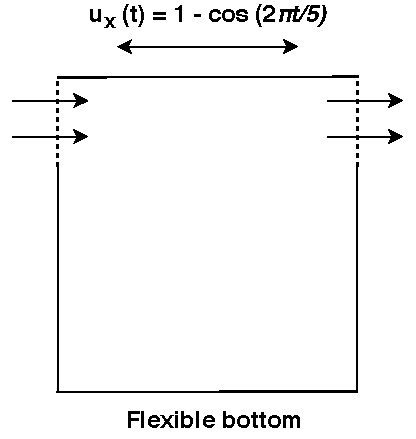
\includegraphics[width=0.43\textwidth,height=0.35\textheight]{images/driven_cavity_geometry.pdf}
\captionsetup{justification=justified}
\caption[2D cross section of driven cavity simulation problem]{Cross section of driven cavity simulation problem with movable bottom wall \cite{driven_cavity}.}
\label{Fig:drivencavity_geometry}
\end{figure}

% \subsubsection{Fluid model}

A cube with dimensions 1 x 1 x 1 meter is the fluid domain of driven cavity. The top surface of the quadratic fluid domain is vertically oscillating a frequency of 0.2 Hertz. The cavity has an inlet and outlet on the top left and top right, respectively, each of width 0.2 meter as illustrated in figure \ref{Fig:drivencavity_geometry}.  The study considers the fluid to be an incompressible fluid with constant density and viscosity \cite{MpCCI_documentation}.

% \subsubsection{Solid model}

The flexible wall is the solid part of the simulation model. The left and right end of the wall is fixed and the wall thickness is 0.002 meters. The results are evaluated at the middle of the bottom flexible wall. The material is considered linearly elastic. The top of the flexible wall aids in exchanging quantities between the solid and fluid domain \cite{MpCCI_documentation}. 

\subsection{Elastic flap in a duct}
\label{section:elastic_flap}
The simulation model includes a rectangular area for fluid domain and the solid structural domain includes in elastic flap. ABAQUS and OpenFOAM are the solid solver and fluid solver respectively used for this simulation problem. The coupling is mediated by MpCCI software package. The geometry of the simulation problem is provided in figure \ref{Fig:elastic_flap}.

\begin{figure}[!ht]
\centering
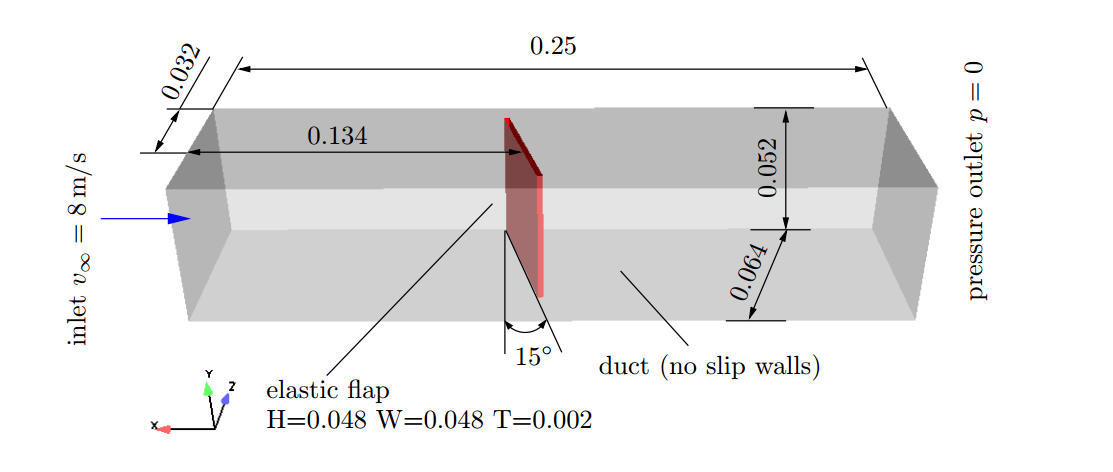
\includegraphics[width=0.78\linewidth,height=0.33\textheight]{images/elasticflap_geometry.png}
\captionsetup{justification=justified}
\caption[Geometry of elastic flap simulation problem]{Geometry and boundary conditions of elactic flap in a duct simulation model \cite{MpCCI_documentation}. The dimensions are provided in meters. The innermost bottom corner of the elastic flap is the control node for computing the results}
\label{Fig:elastic_flap}
\end{figure}

% \subsubsection{Fluid model}

The entire cuboid area excluding the elastic flap corresponds to the fluid domain. An incremental time step of 0.25 millisecond is used by the computational fluid dynamics- fluid solver code. 

% \subsubsection{Solid model}

The red colored rectangle corresponds to the solid surface. The elastic flap is a linearly elastic material. The solid has been divided into mesh grids for computation with 20 nodes for each mesh. The top surface nodes are stationary. An adaptive time step is used with an incremental time step of 0.25 millisecond up to 0.2 seconds.  The innermost bottom corner of the elastic flap is the control node for computing the results. In this problem, the quantity time step is coupled in the coupling region.

\subsection{Significance of hyperparameters}

An extensive description on the steps involved in designing and conducting the simulation is provided in the MpCCI manual- chapter Tutorial \cite{MpCCI_documentation}. In order to explain the importance of the hyperparameter involved in the research project, 3D driven cavity simulation problem is considered. On performing the simulation using MpCCI, the moving surface at the top results in an oscillating bottom wall.  

\begin{figure}[!ht]
\centering
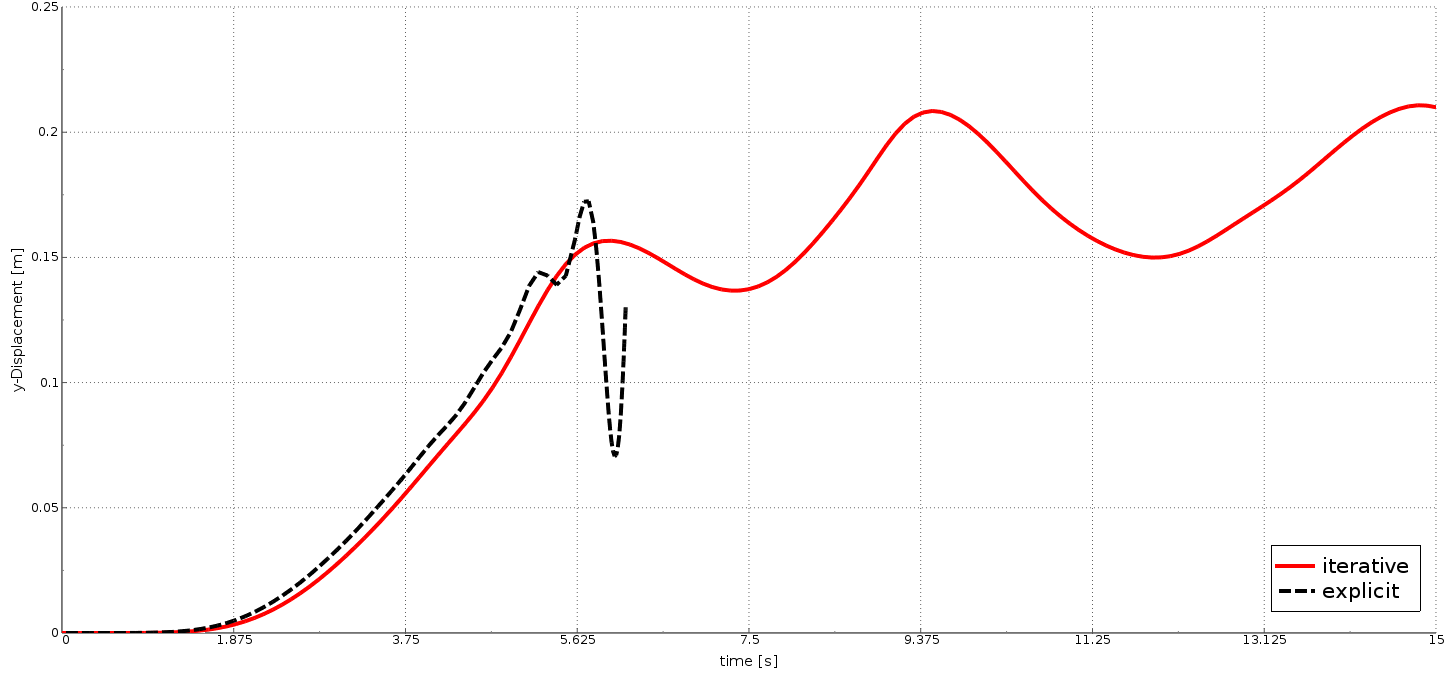
\includegraphics[width=\textwidth]{images/driven_cavity_result1.png}
\captionsetup{justification=justified}
\caption[An illustration of the significance of hyperparameters]{Impact of 'Coupling scheme' hyperparameter in driven cavity- Iterative transient coupling versus explicit coupling for 3D driven cavity \cite{MpCCI_documentation}. The simulation will fail on configuring the coupling scheme with explicit coupling.}
\label{Fig:iterative_vs_explicit}
\end{figure}

The figure \ref{Fig:iterative_vs_explicit} illustrates on solving the driven cavity problem using explicit coupling scheme diverges the solution. However, the iterative implicit coupling leads to convergence and stable oscillations \cite{MpCCI_documentation}. 

% \begin{figure}[!ht]
% \centering
% 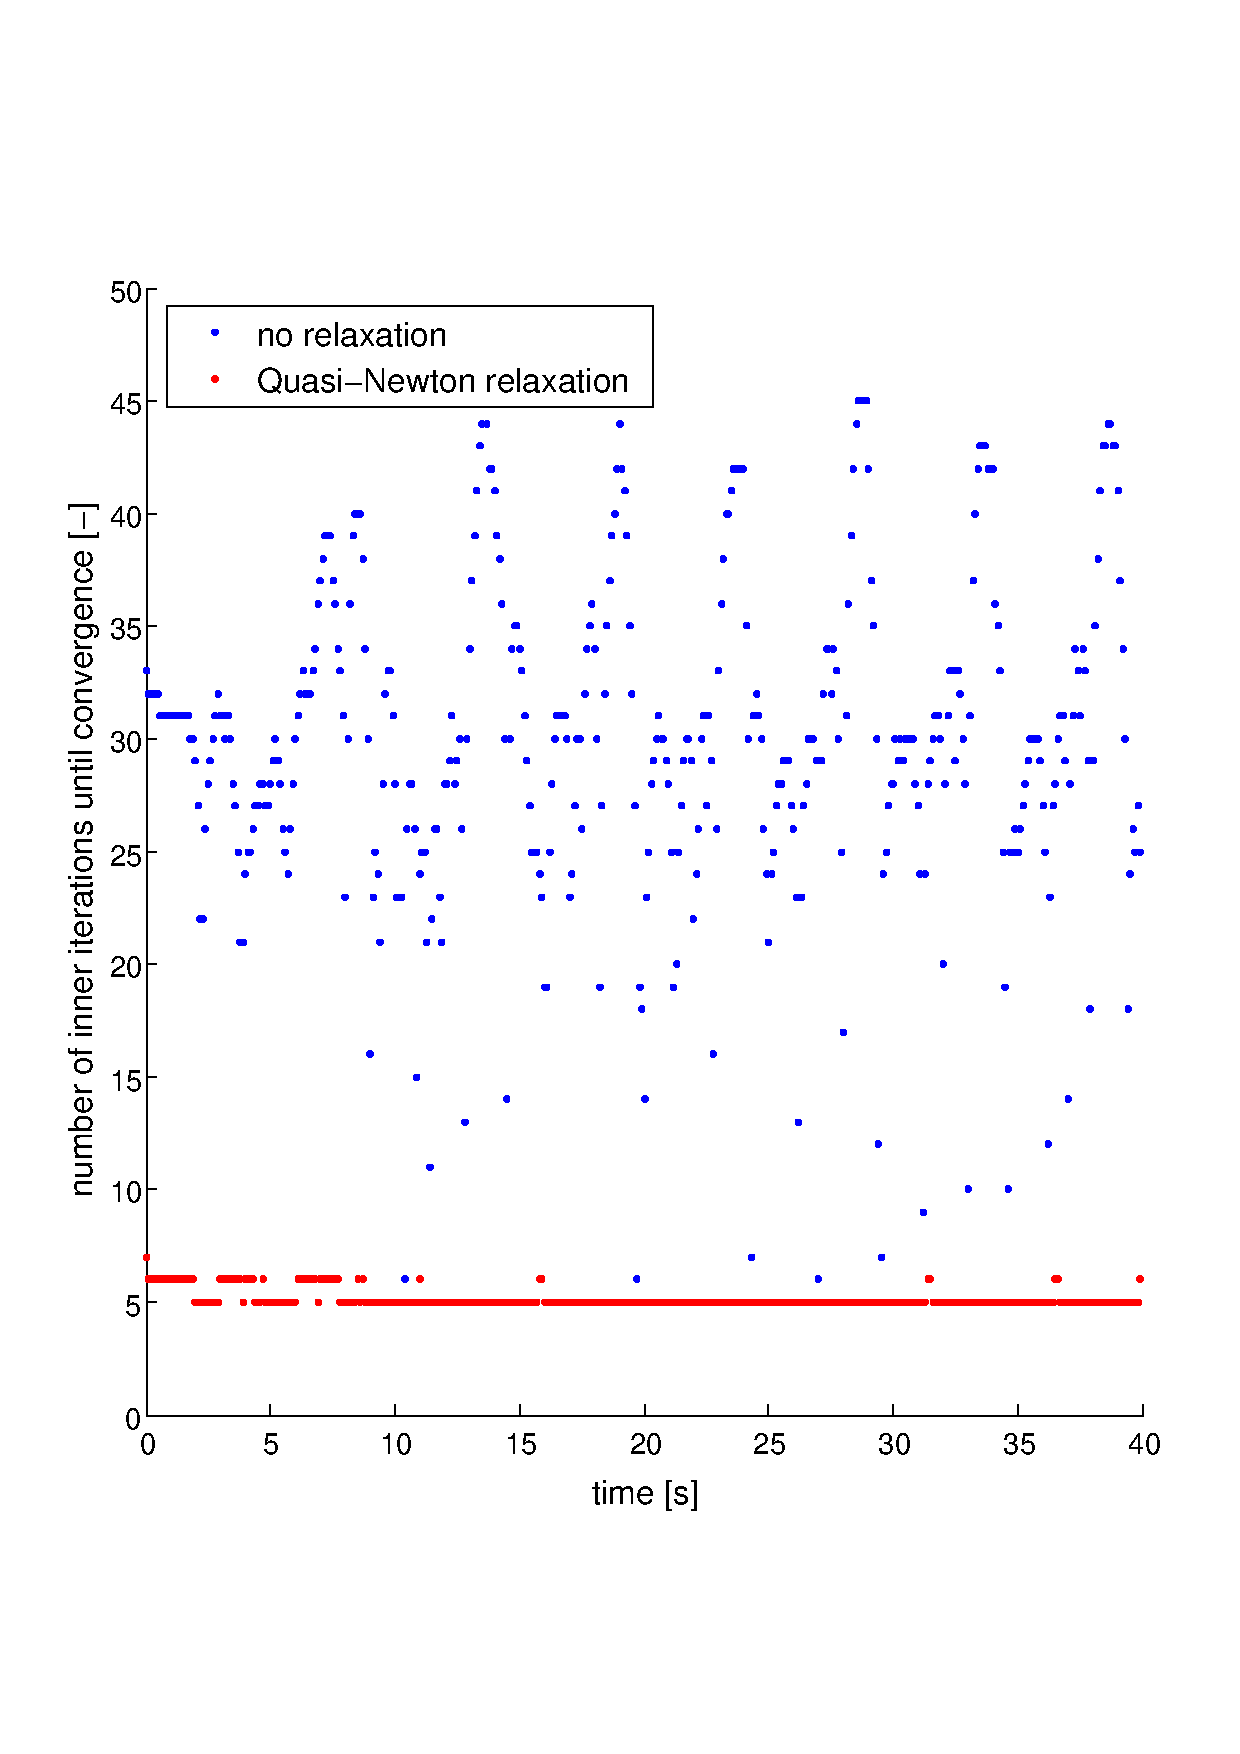
\includegraphics[trim={0 5cm 0 3cm},clip,width=0.78\textwidth,height=0.5\textheight]{images/qn_relaxation_drivencavity_2.pdf}
% \captionsetup{justification=justified}
% \caption[Effectiveness of Quasi-Newton relaxation method for 3D-driven cavity]{Comparison of convergence at each time step using iterative coupling scheme \cite{MpCCI_documentation}. }
% \label{Fig:qn_relaxation}
% \end{figure}
%  trim={<left> <lower> <right> <upper>}
\begin{figure}[!h]
\centering
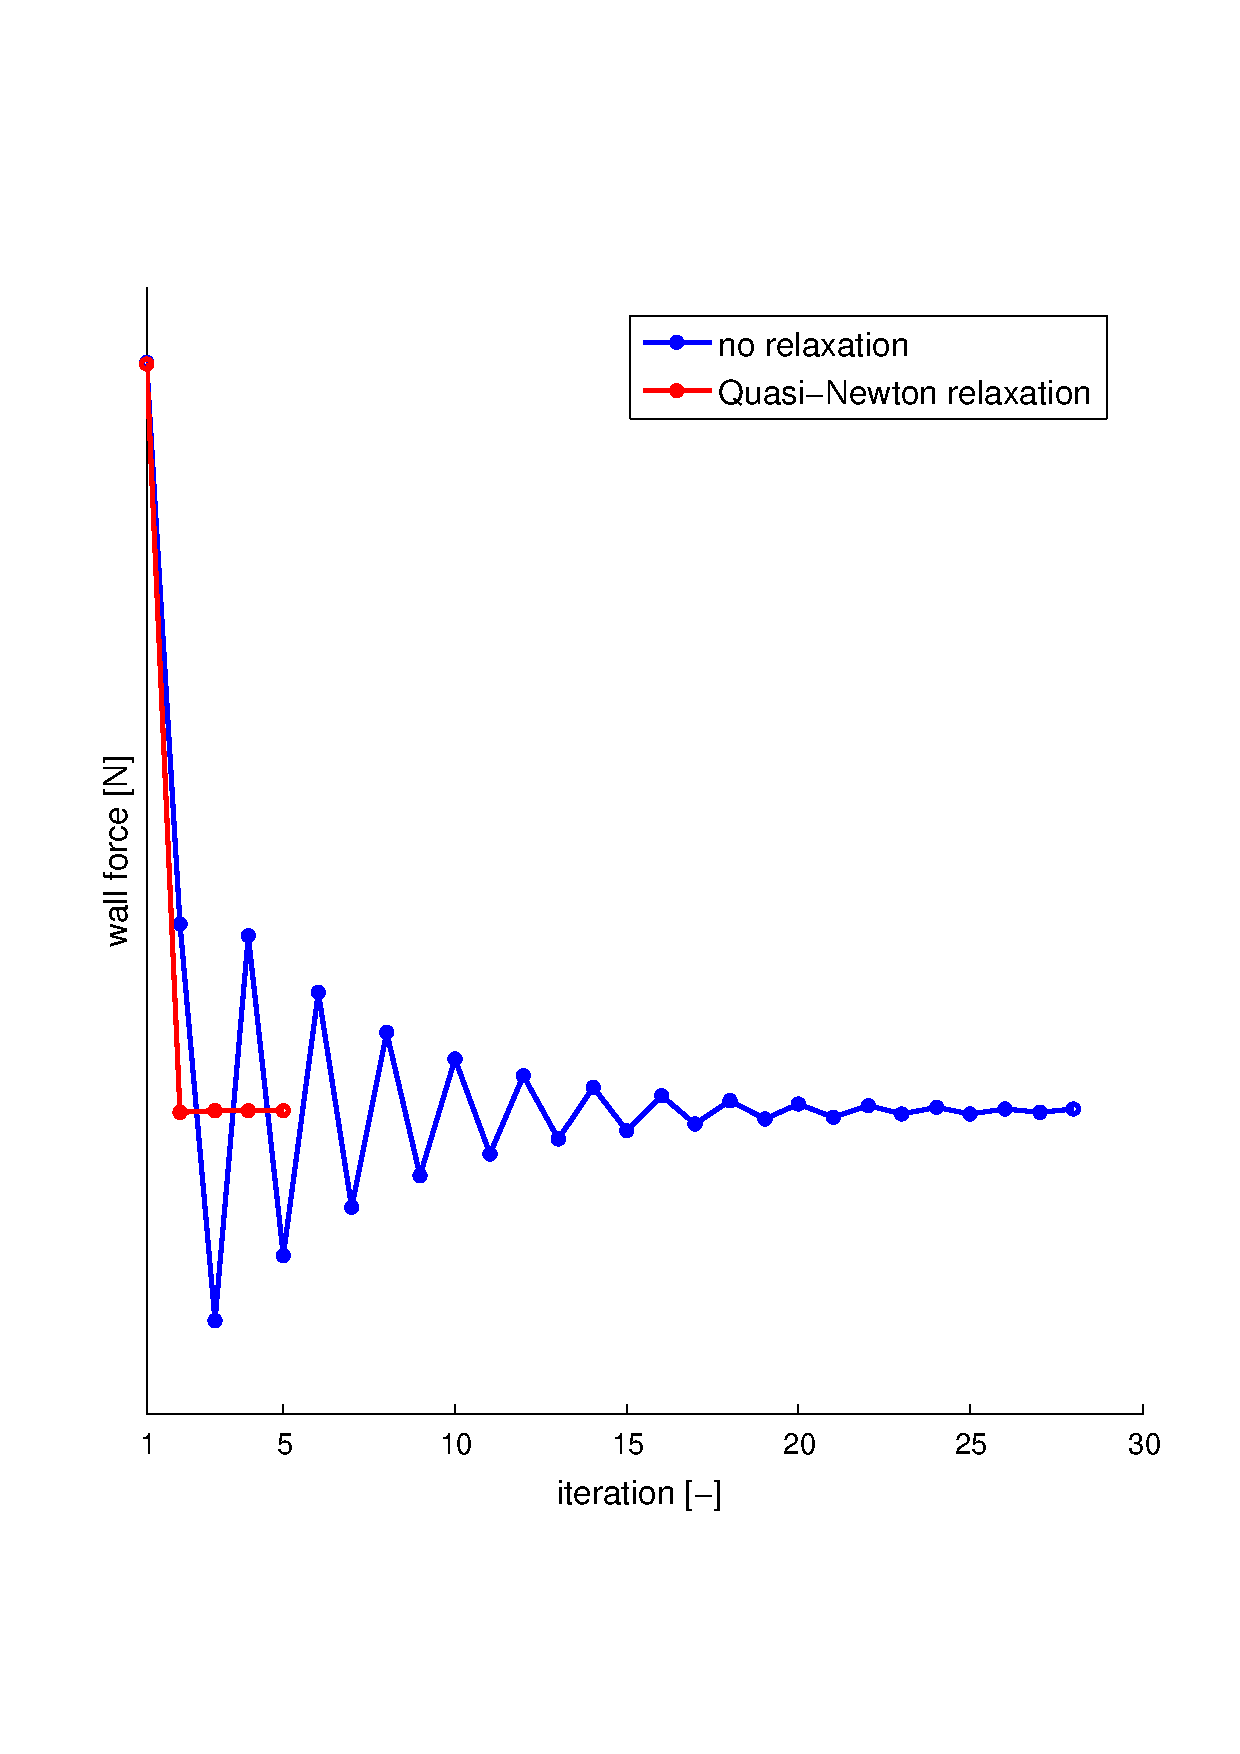
\includegraphics[trim={0 3cm 0 3cm},clip,width=0.66\textwidth,height=0.47\textheight]{images/qn_relaxation_drivencavity_1.pdf}
\captionsetup{justification=justified}
\caption[Effectiveness of Quasi-Newton relaxation method for 3D-driven cavity]{Effectiveness of Quasi-Newton relaxation method for 3D-driven cavity \cite{MpCCI_documentation}.}
\label{Fig:qn_relaxation}
\end{figure}

The iterative transient coupling scheme solves the simulation in 20.5 hours. On testing the effect of Quasi-Newton relaxation method, the time factor is reduced by seven and the oscillations of each iteration is eliminated as illustrated in figure \ref{Fig:qn_relaxation} \cite{MpCCI_documentation}.


\section{Smart coupling tool}
\label{chapter:implementation}

The research work contributes to the engineers and researchers performing simulation studies by providing two significant implementations- smart coupling tool and feature reader tool.

Smart coupling is the process of automatically configuring the coupling tool using algorithm configuration methods. The development of the smart coupling tool is divided into 4 phases- Optimization \ref{section:optimization_phase}, data pre-processing \ref{section:data_preprocessing}, training \ref{section:training_phase} and prediction phase \ref{section:prediction_phase}.

The feature reader tool is a separate python-based package. It is used by the smart coupling tool to extract features from the simulation model files, coupling tool input files, and output files. The appendix \ref{appendix:gitlab_package} provides the step-by-step instructions to use the smart coupling tool and feature reader package. 

\subsection{Feature reader}
\label{section:feature_reader}

The features of the simulation problem integrate the characteristics of the following components of the simulation,

\begin{itemize}
\item The simulation models- solid and fluid model.
\item The coupling method.
\end{itemize}

The characteristics of the simulation models include – density of the fluid, the density of the solid structure, elasticity of the solid, viscosity of the fluid, Poisson's ratio, and the ratio of solid-fluid density, and type of the simulation problem- stationary or transient study.   The characteristics of the coupling method include the coupling type, time step, number of nodes in the coupling region, tolerance of each time step, and the time taken for the co-simulation.

The feature reader package is used to extract approximately more than 100 features covering the entire domain of FSI simulations. This package requires the input simulation code files, coupling code files, and the coupling result-log file of the simulation process. The smart coupling tool utilizes feature reader to enrich the surrogate model by providing the features of the simulation instances.

\subsection{Optimization phase based on SMAC}
\label{section:optimization_phase}

The integral part of the optimization phase is Sequential Model-based Algorithm Configuration (SMAC). SMAC is a variant of Bayesian optimization. This section explains the optimization phase elements. The figure \ref{fig:optimization} illustrates the optimization phase. The components of the optimization phase are provided below.

\begin{itemize}
\item Inputs to SMAC: The inputs include the simulation instances and features of the instances.
\item Configuration space of the MpCCI configurable parameters. The description of the parameters are provided in section \ref{section:hyperparameters_couplingtool}. 
\item Outputs of SMAC: The various allowable configurations to perform coupling simulations, cost (runtime in seconds) on executing the target algorithm with the respective configuration, and the features of the simulation instances. The outputs of SMAC comprise the dataset for training the machine learning models to predict the optimal configurations.
\end{itemize}

\begin{figure}[!ht]
\centering
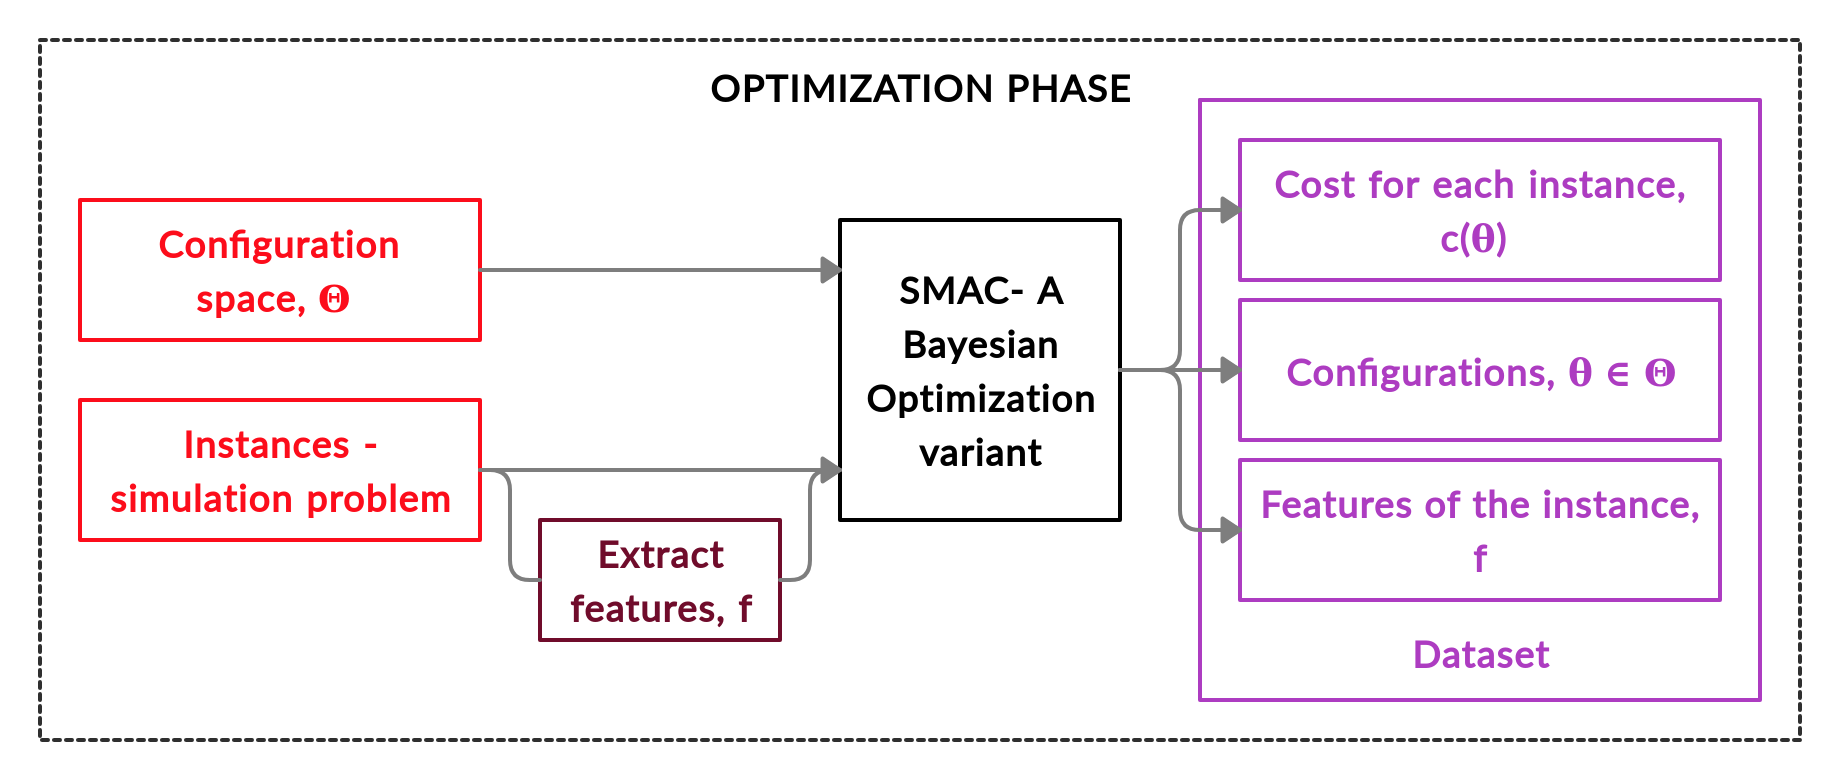
\includegraphics[width=0.9\linewidth,height=0.4\textheight]{images/Optimizationphase.jpg}
\captionsetup{justification=justified}
\caption[Optimization phase- Block diagram]{Block diagram of optimization phase. The inputs (red) are the configuration space and various simulation instances. The feature is extracted using the feature reader tool (brown). SMAC (black) performs single instance optimization of the simulation problems resulting in a multiphysics simulation dataset (purple).}
\label{fig:optimization}
\end{figure}

\subsubsection{Simulation instances}
A simulation instance is a particular occurrence, case, or example of a simulation problem. In this research, various simulation instances are developed by varying the solid and fluid model features of a particular simulation problem. The simulation problems taken into consideration are the 3d driven cavity and elastic flap. The simulation problems are discussed in section \ref{section:simulation_problem}. A total of 19 instances are developed by varying the features, namely- elasticity, solid density, Poisson's ratio, fluid density, and fluid viscosity. The features of the instances are provided in tables \ref{table:simulationinstances_train} and \ref{table:simulationinstances_evaluation}. The features are used to enhance the RF surrogate model of SMAC. However, SMAC optimizes the simulation instances considering the instances as a black-box.

\subsubsection{Configuration space of the parameters}
\label{section:configurationspace}

The configuration space, $\Theta$ is the vector space spanned by the parameters defining the states of a target algorithm, $\mathcal{A}$. The target algorithm in this research work is the coupling tool, MpCCI. A parameter configuration, $\theta \in \Theta$, is evaluated on a particular instance 'i' of the target algorithm resulting in $\mathcal{A}$($\theta$). Each target algorithm evaluation is associated with a performance metric, 'm'. This metric characterizes the behavior of the target algorithm for a particular pair of parameter configuration and instance.


\begin{table}[htbp]
\footnotesize
\begin{center}
\begin{tabular}{|l|l|l|}
\hline
\textbf{Parameter, P} & \textbf{Parameter type} & \textbf{Domain of the parameter, D} \\ \hline
Coupling scheme & Categorical &\makecell[l]{Implicit-Transient:Implicit-Transient,\\Explicit-Transient:Explicit-Transient} \\ \hline
Initial exchange & Categorical & \makecell[l]{exchange:exchange, receive:exchange, \\exchange:receive}  \\ \hline
Relaxation-0 & Categorical & True, False \\ \hline
Relaxation-1 & Categorical & True, False \\ \hline
Relaxation method & Categorical & Quasi-Newton, Fixed, Aitken, Ramping \\ \hline
Anderson mix& Categorical & Least squares, Standard, Inverse \\ \hline
Number of levels  & Integer & [0, 16] \\ \hline
Omega & Float & [1e-07, 2.0] \\ \hline
Ramp-0 & Float & [0.0, 2.0] \\ \hline
Ramp-d & Float & [0.001,1.0] \\ \hline
Relaxation factor & Float & [0.0,2.0] \\ \hline
\end{tabular}
\end{center}
\captionsetup{justification=justified}
\caption[Hyperparameters of the coupling tool]{Hyperparameters of the coupling tool.}
\label{table:parametertypes}
\end{table}

This section provides the parameter involved in the study, type of the parameters, domain of the parameter, and the conditional dependencies among the parameters. The following table \ref{table:parametertypes} summarizes the various parameters used in the study, the domain of the parameters, and the parameter types.  The domain of a parameter is the set of acceptable values for a parameter \cite{Hutterphd}. An overview of the various data types of parameters is provided in section \ref{section:AACmindmap}. In FSI, QN is the most efficient and robust relaxation method for partitioned coupling \cite{robustqn} \cite{robustqn2}. The following default parameter values are used in MpCCI for QN based problems.


\begin{table}[htbp]
\begin{center}
\begin{tabular}{|l|l|}
\hline
\textbf{Parameter, P} & \textbf{Default value} \\ \hline
Coupling scheme & Implicit-Transient:Implicit-Transient\\ \hline
Initial exchange & receive:exchange \\ \hline
Relaxation\_0 & False  \\ \hline
Relaxation\_1 & True  \\ \hline
Relaxation method & Quasi-Newton \\ \hline
Andersonmix type & Inverse  \\ \hline
Number of levels  & 1 \\ \hline
Omega & 0.1  \\ \hline
Ramp\_0 & 0.1 \\ \hline
Ramp\_d & 0.1 \\ \hline
Relaxation factor & 0.1 \\ \hline
\end{tabular}
\end{center}
\captionsetup{justification=justified}
\caption[Default parameter configuration of MpCCI]{Default configuration majorly used in MpCCI.}
\label{table:parameterdefaultvalues}
\end{table}

The conditional parameter clauses define the conditional parameters. The two components of a conditional parameter clause are the child parameter and a logical condition with parent parameters. On the parent parameter satisfying the logical condition, the child parameter is considered for parameter setting \cite{Hutterphd}. The table \ref{table:conditionalparameters} summarize the conditional parameters in this study. 

\begin{table}[htbp]
\begin{center}
\begin{tabular}{|r|l|l|}
\hline
\multicolumn{1}{|p{3cm}|}{\centering \textbf{Conditional\\Clause}} & \textbf{Child parameter} & \textbf{Parent logical condition} \\ \hline
1 & Relaxation method & \begin{tabular}{@{}@{}}Relaxation\_0 == True $||$\\ Relaxation\_1 == True \end{tabular}  \\ \hline
2 & Andersonmix type & Relaxation method == Quasi-Newton \\ \hline
3 & Number of levels & Relaxation method == Quasi-Newton \\ \hline
4 & Omega & Relaxation method == Quasi-Newton \\ \hline
5 & Relaxation factor & Relaxation method == Fixed \\ \hline
6 & Ramp\_0 & Relaxation method == Ramping \\ \hline
7 & Ramp\_d & Relaxation method == Ramping \\ \hline
\end{tabular}
\end{center}
\captionsetup{justification=justified}
\caption[Conditional parameters of the study]{Conditional parameters of the study.}
\label{table:conditionalparameters}
\end{table}

Furthermore, the forbidden clauses in SMAC allow specifying the restricted parameter configurations. Condition 1 and condition 2 is a pair of invalid parameter configuration. The configurator does not evaluate the target algorithm with the forbidden configurations provided in table \ref{table:forbiddenconditions}.  

\begin{table}[htbp]
\begin{center}
\begin{tabular}{|r|l|l|}
\hline
\multicolumn{1}{|p{2cm}|}{\centering \textbf{Forbidden\\ Clause}} & \textbf{Condition 1} & \textbf{Condition 2} \\ \hline
1 & Relaxation\_0 == True & \begin{tabular}{@{}@{}}Coupling scheme == Explicit-Transient:\\ Explicit-Transient \end{tabular} \\ \hline
2 & Relaxation\_1 == True & \begin{tabular}{@{}@{}}Coupling scheme == Explicit-Transient:\\ Explicit-Transient \end{tabular}\\ \hline
3 & \begin{tabular}{@{}@{}}Initial exchange ==\\ exchange:exchange \end{tabular}& \begin{tabular}{@{}@{}}Relaxation\_0 == True \&\&\\ Relaxation\_1 == True \end{tabular}   \\ \hline
4 &  \begin{tabular}{@{}@{}}Initial exchange ==\\ exchange:exchange \end{tabular} & \begin{tabular}{@{}@{}}Relaxation\_0 == False \&\&\\ Relaxation\_1 == True \end{tabular} \\ \hline
5 & \begin{tabular}{@{}@{}}Initial exchange ==\\ exchange:exchange \end{tabular} & \begin{tabular}{@{}@{}}Relaxation\_0 == True \&\&\\ Relaxation\_1 == False \end{tabular}\\ \hline
\end{tabular}
\end{center}
\captionsetup{justification=justified}
\caption[Forbidden pairs of parameter configuration]{Forbidden pairs of parameter configuration.}
\label{table:forbiddenconditions}
\end{table}

The nature of a configuration space of the parameters, $\Theta$ is primarily determined by the number of parameters, parameter types, the domain of the parameters, constraints of the parameter configurations, and the various conditional parameters involved in the algorithm configuration problem. The algorithm for searching the optimal configurations are decided depending on the configuration space of the parameters. An algorithm configuration procedure, SMAC performs the process of exploring the configuration space for optimal parameter configuration of a given instance \cite{Hutterphd}. 

\subsubsection{Single instance optimization by SMAC}
\label{section:smac}
SMAC is a variant of BO with the RF surrogate model. The regression model to fit the sample points is a RF regressor. The major contributions of SMAC are eliminating the two major disadvantages of Sequential Model-Based Optimization (SMBO) discussed in section \ref{section:model-based}, namely the restriction of SMBO for target algorithms with numerical parameters and single instance optimization of the target algorithm \cite{SMAC_mainpaper}.

SMAC utilizes RF for modeling the objective function. The objective function or target algorithm is MpCCI in this research. RF handles categorical parameters efficiently \cite{Hutterphd} by providing an increased performance because of the set of decision trees in the forest \cite{SMAC_mainpaper} \cite{RF_mainpaper}. RF incorporates a group of regression trees predicting the performance metric of MpCCI. The regression tree prediction depends on the knowledge of the evaluations at a particular point in the optimization task.

The second significant advantage of SMAC is the ability to handle multiple instances. The set of parameter configurations, the respective performance metric obtained by evaluation of the parameter configuration on instance $i$, and the respective feature $f$ of the instance $i$, is used to train the RF model.

AutoML Group, University of Freiburg, provides the algorithm configuration tool- SMAC3 \cite{smac-github}. An extended algorithm of the smart coupling tool integrating the algorithm of SMAC is provided in algorithm \ref{algo:smac}. 

\subsection{Data pre-processing}
\label{section:data_preprocessing}
The data pre-processing focus on the transformation of the cost metric, followed by normalization with the minimum cost of the simulation instance.

The cost metric of the optimization task is the runtime (in seconds). The runtime provides large variations in the dataset. The various previous works on runtime prediction recommend logarithmic transformation of the runtime because logarithmic transformation aids in runtime prediction by reducing the dynamic range of the runtime \cite{SMAC_mainpaper} \cite{SMAC_extendedpaper}. In addition to logarithmic transformation in equation \ref{equation:log}, the results are compared using scaled-logarithmic (equation \ref{equation:log-scaled}) and scaled-inverse (equation \ref{equation:inverse-scaled}) transformations. All the transformations are adapted from \cite{smac-github}.

Logarithmic transformation:
\begin{equation}
    Tc(\theta_{i}, f_j) = \ln\left(c(\theta_{i}, f_j)\right)
    \label{equation:log}
\end{equation}

Scaled-logarithmic transformation:
\begin{equation}
    Tc(\theta_{i}, f_j) = \ln \left(\frac{c(\theta_{i}, f_j)-min[c(\theta, f_j)]+\epsilon }{max[c(\theta, f_j)]-min[c(\theta, f_j)] +\epsilon}\right)
    \label{equation:log-scaled}
\end{equation}

Scaled-inverse transformation:
\begin{equation}
    Tc(\theta_{i}, f_j) =1- \left( \frac{c(\theta_{i}, f_j)-max[c(\theta, f_j)]}{c(\theta_{i}, f_j)-min[c(\theta, f_j)] +\epsilon}\right)^{-1}
    \label{equation:inverse-scaled}
\end{equation}

c($\theta_{i}$, $f_j$) and Tc($\theta_{i}$, $f_j$) are the cost metric for the configuration $\theta_i$ of a particular simulation instance j with feature set $f_j$ before and after transformation, respectively.  min[c($\theta, f_j$)] and max[c($\theta, f_j$)] is the minimum and maximum cost respectively for a particular simulation instance j with the feature set $f_j$ over all the parameter configurations. The variables i and j ranges up to the total iterations of SMAC and total instances in the training set, respectively. $\epsilon$, a very small constant, is added to the minimum of the cost vector for a particular instance to avoid division by zero issues.

The simulation instances in table \ref{table:simulationinstances_train} differ by the features. The different features cause variations in the simulation time for different parameter configurations of the coupling tool. The transformed cost of each simulation instance is normalized with the minimum cost of a particular simulation instance to make the features comparable concerning the cost metric.

\begin{equation}
    c_n(\theta_{i}, f_j) = \frac{Tc(\theta_{i}, f_j)}{min[Tc(\theta, f_j)]}
\end{equation}

Tc($\theta_{i}$, $f_j$) and $c_n$($\theta_{i}$, $f_j$) are the transformed and normalized cost, respectively, for the configuration $\theta_i$ of a particular simulation instance j with feature set $f_j$.  min[Tc($\theta, f_j$)] is the minimum of the transformed cost for a particular simulation instance j with the feature set $f_j$ over all the parameter configurations.

% Why transformation- https://scikit-learn.org/stable/auto_examples/compose/plot_transformed_target.html#sphx-glr-auto-examples-compose-plot-transformed-target-py

\subsection{Training phase}
\label{section:training_phase}
At the end of the optimization phase, the dataset for training machine learning models to predict optimal configurations is available. The optimal configurations are predicted using two different models, namely configuration and cost response models. The labels of the configuration and cost response models are the parameter configurations and costs, respectively. The figure \ref{fig:config_response} and figure \ref{fig:cost_response} illustrates the pre-processing, training and prediction steps of a configuration and cost response model, respectively.

In configuration response models, the machine learning models- RF, KNN, SVM, GBM, and QRF are trained to predict each of the configurations performing multi-target regression. The method is implemented using the sklearn API \cite{sklearn_api} employing one regressor per target variable. The cost metric is transformed and normalized with the minimum cost similar to the process described in section \ref{section:data_preprocessing}. 

\begin{figure}[!ht]
\centering
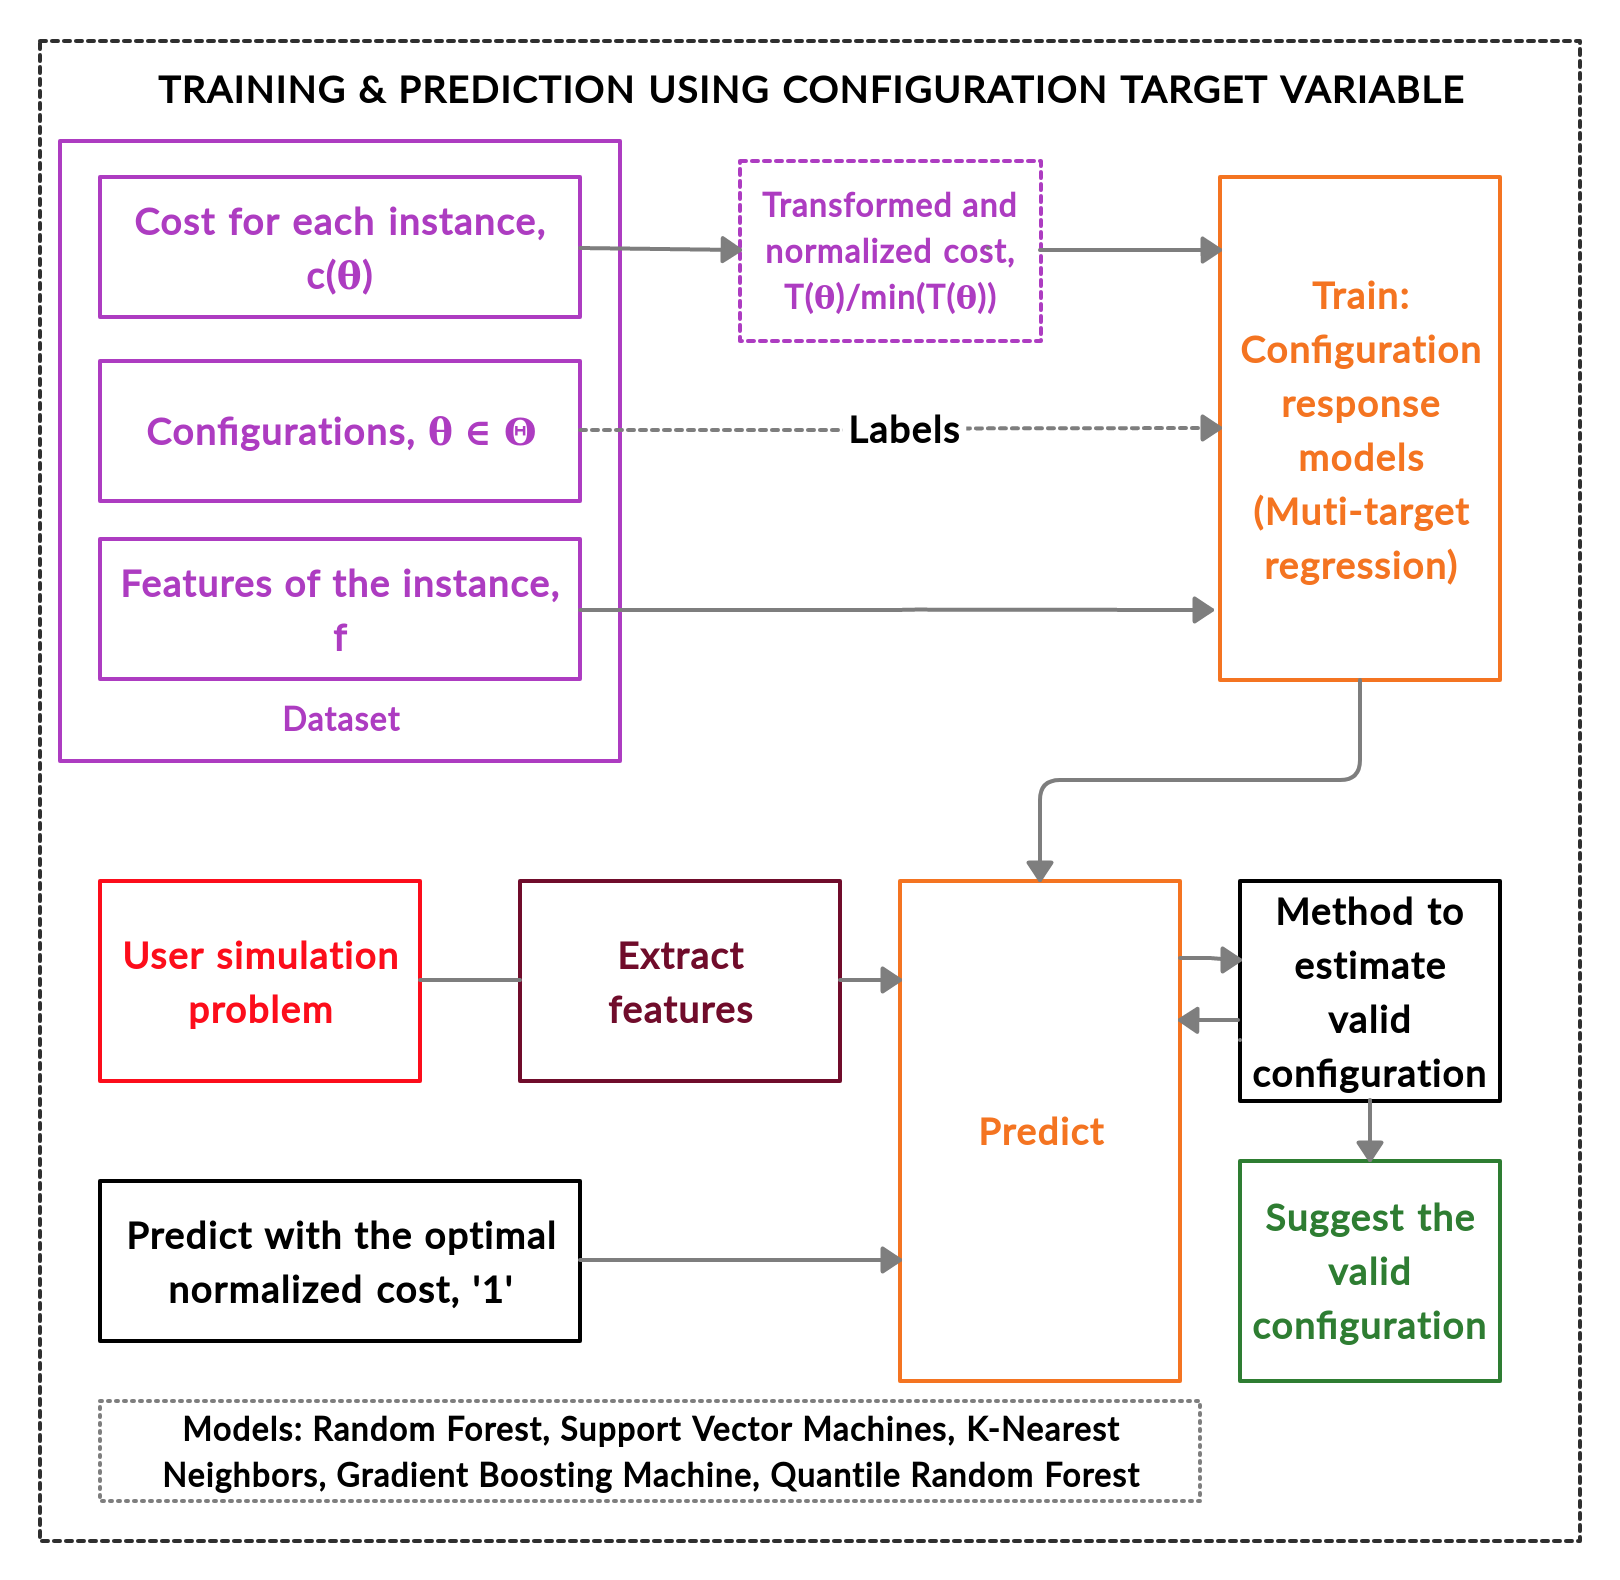
\includegraphics[width=0.9\linewidth,height=0.6\textheight]{images/configuration_response.jpg}
\captionsetup{justification=justified}
\caption[Configuration response model training and prediction phase]{Illustration of the configuration response models (orange) training and prediction phase. The labels (dashed line) of configuration response models are the parameter configurations of the dataset (purple). The cost is transformed and normalized in the data pre-processing step (dashed purple) with the respective transformations discussed in \ref{section:data_preprocessing}. The prediction for the user given FSI simulation problem (red) occurs at optimal normalized cost value 1 because the optimal cost value for a particular feature set is 1 during training phase. The method after prediction check for valid configuration and predict with an incremented normalized cost value up to a threshold searching for valid predictions. The feature reader tool is used to extract features (brown) during prediction.}
\label{fig:config_response}
\end{figure}

In cost response models, the machine learning models- RF, KNN, SVM, GBM, and QRF are trained to predict the cost metric of the simulation instance. The configurations and features of the simulation instance in the dataset are the features to train the model. The transformed and normalized cost is the label. In addition to the above-specified models, RF is trained to predict the expected improvement metric of a particular configuration. It is included in the cost response models because EI indicates the utility of a configuration. RF-EI indicates the RF model predicting expected improvement in the upcoming sections.

\begin{figure}[!ht]
\centering
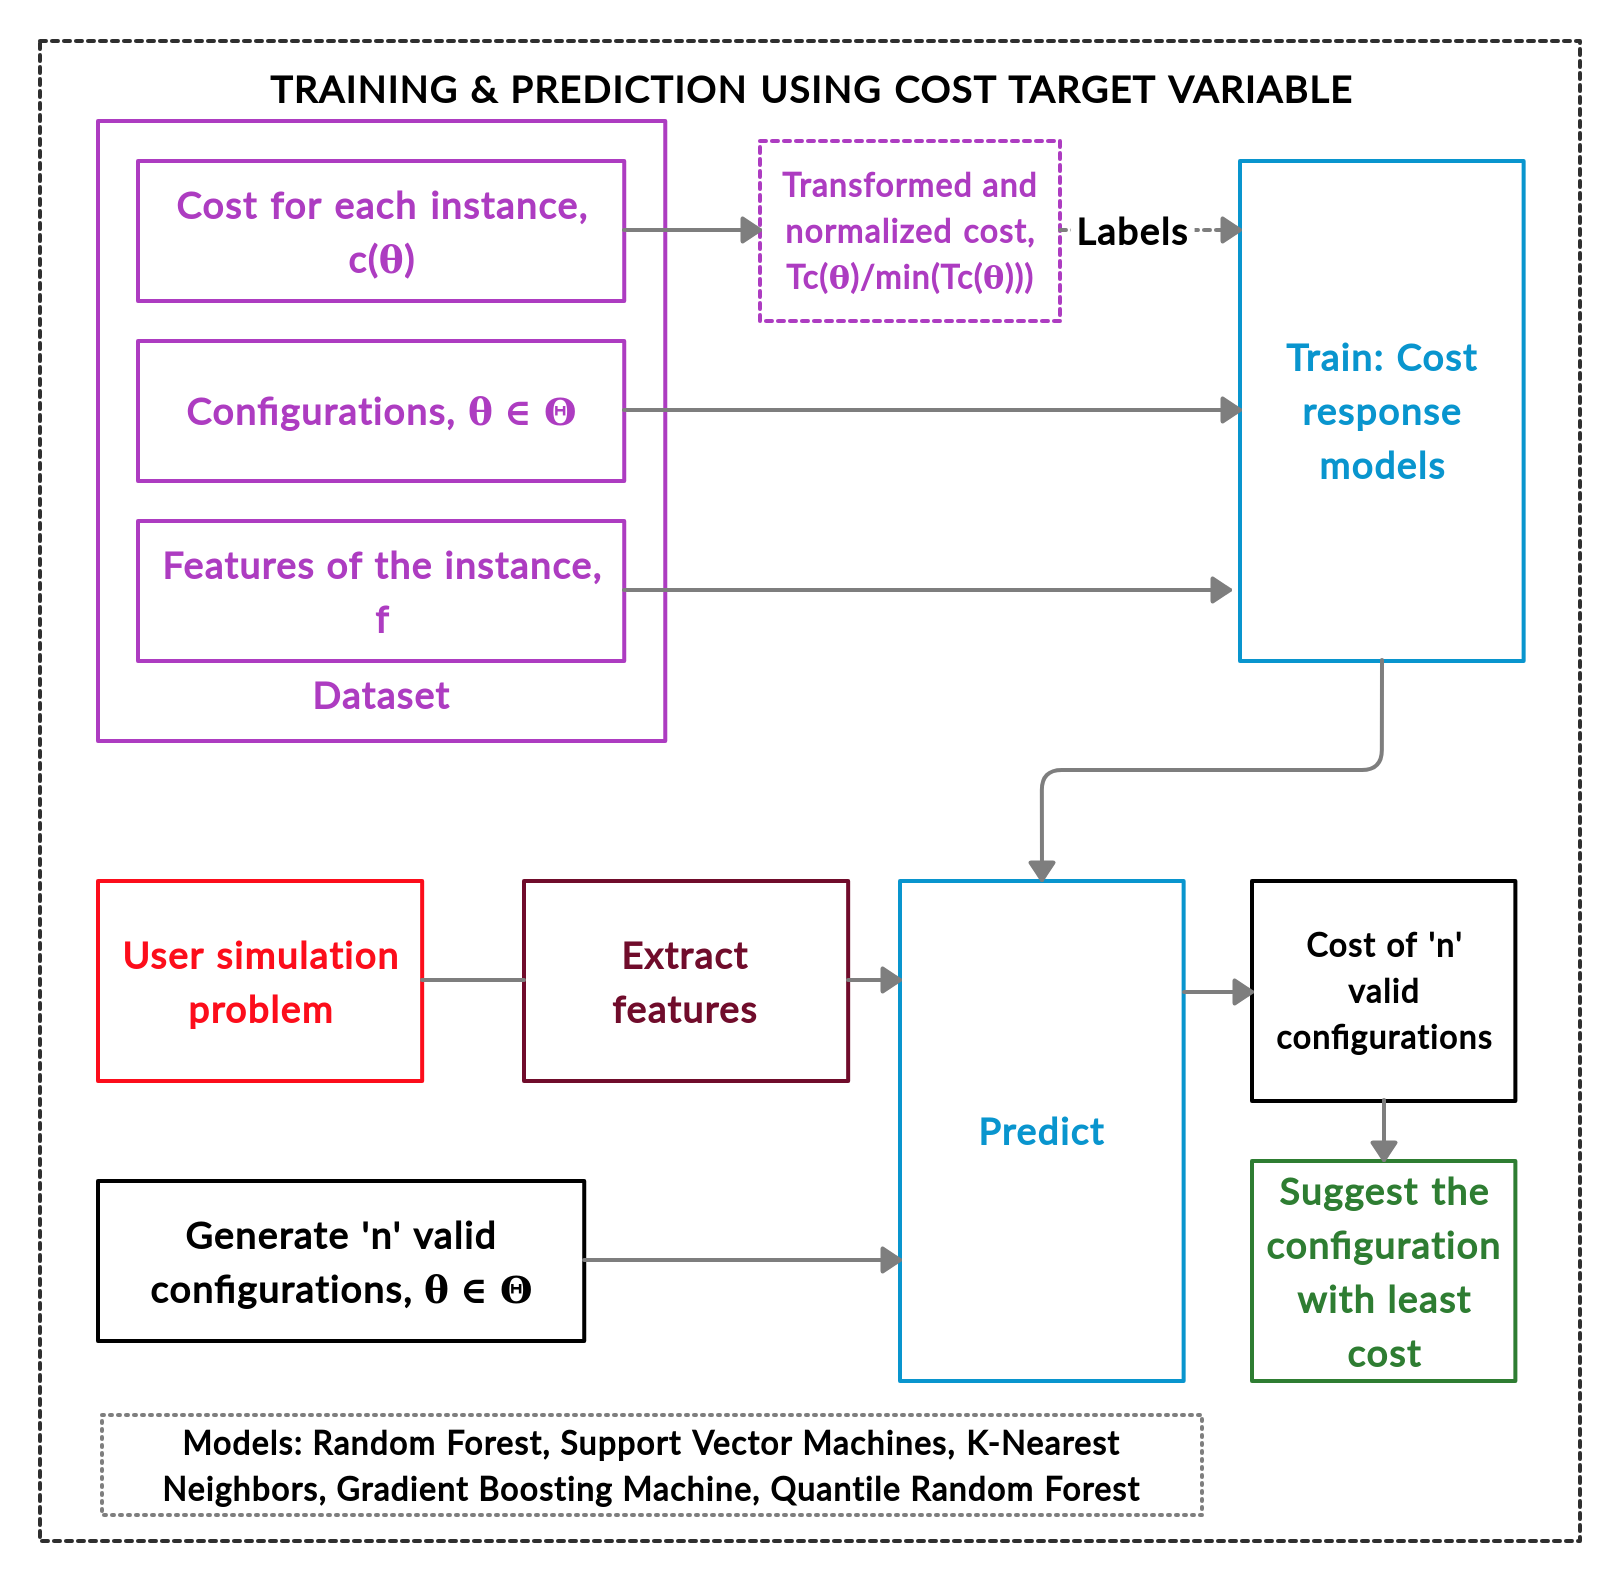
\includegraphics[width=0.9\linewidth,height=0.6\textheight]{images/cost_response.jpg}
\captionsetup{justification=justified}
\caption[Cost response model training and prediction phase]{Illustration of the cost response models (blue) training and prediction phase. The labels (dashed line) of the cost response models are cost. The dataset (purple) is the multiphysics dataset developed by optimization. The cost is transformed and normalized in the data pre-processing step (dashed purple) with the respective transformations discussed in \ref{section:data_preprocessing}. The prediction for the user given FSI simulation problem (red) involves the generation of numerous valid configurations followed by predicting the configuration with desirable least cost (green) for a particular simulation instance. The feature reader tool is used to extract features (brown) during prediction.}
\label{fig:cost_response}
\end{figure}

\subsection{Prediction phase}
\label{section:prediction_phase}

The prediction procedure of configuration and cost response models are illustrated in figures \ref{fig:config_response} and \ref{fig:cost_response}. The prediction phase of both response models incorporates the feature reader tool to extract features from the user-provided simulation problem.

In configuration response models, the prediction begins with cost value 1 because the optimal cost pertaining to a particular feature set is 1. This is primarily due to the normalization with the minimum cost of a particular instance. The configuration is predicted as a vector of floating-point values for the user given feature set. The floating-point predictions for categorical parameters are rounded to the nearest integer to map the predictions to the closest category. This configuration is not assured to be a valid configuration because of the conflict with the forbidden and conditional parameters. Therefore, a method predicts the configurations with an incremented cost value until the predictor estimates a valid configuration. This new incremented cost value is a sub-optimal cost. This is implemented in the method after the prediction block. Finally, the valid configurations are suggested to the user.

In cost response models, the prediction phase incorporates the generation of numerous random valid configurations. The predictor predicts the cost metric for a particular feature provided by the user using all the random configurations generated. Finally, the parameter configuration with the least cost is proposed to the user.

The performance of each model is analyzed in the experiments and results section \ref{chapter:experimentation_results}. Finally, the user is suggested with the top 3 configurations predicted by 3 models out of the 11 configuration and cost response models.

\subsection{Workflow of the smart coupling tool developed}
\label{section:smac_smartcoupling_algorithm}

The workflow of the smart coupling tool revolves majorly around the working of SMAC. The working of SMAC is similar to the BO procedure with the gaussian surrogate model provided in the algorithm \ref{algo:bayesianopt} with changes in the surrogate model training followed by configurations selection and intensification. The outputs from SMAC by single instance optimization is used for training and predicting the optimal configuration. The workflow of smart coupling is enumerated below.

\begin{enumerate}
\item \textbf{Define the inputs:} SMAC requires a set of training instances $i$, configuration space $\Theta$, and features of the training instances $x_i$. Furthermore, the default configuration $\theta_{default}$ for all instances, the forbidden parameter configuration cases, conditional dependencies of the hyperparameters, the seed for generation of random configurations are provided. 

\item \textbf{Evaluate the default configuration:} The optimization of each instance begins with the target algorithm evaluation using the default configuration. This can be altered depending on user requirements. The wrapper performing the evaluation estimates the performance metric associated with the evaluation, $R_i$. The default configuration is the current best configuration for the first iteration with the best cost $\theta_{i,inc}$. The best configuration at any point in the program is called incumbent configuration. At each iteration, $\theta_{i,inc}$, and the associated best cost, $c_{i,inc}$ is modified depending on the performance of the new configuration.

\item \textbf{Fit surrogate model:} The training set of the surrogate model includes the parameter configurations and the features specific of a particular instance to predict the cost. This joint model aids in learning the optimal configurations for a particular feature set of the problem. The mean across all the trees is the predicted performance metric for a particular instance and parameter configuration. The variance across all the trees is the uncertainty measure associated with a particular prediction. The cost metric relating to the runtime of the simulation is transformed using logarithm transformation. This reduces the variance in the runtime and improves model performance in the regression task \cite{SMAC_mainpaper} \cite{SATZILLA}. 

\item \textbf{Select configurations:} 
The expected improvement score (EI) is estimated for randomly generated 5000 configurations depending on the surrogate model distribution. The top 50 configurations concerning EI scores are selected to be the challengers of the current best configuration. EI score is high for configurations with low cost metric and high uncertainty \cite{SMAC_mainpaper} \cite{SMAC_extendedpaper}.  

From the second iteration of SMAC, the algorithm performs local search initialized at each of the top 10 promising configurations depending on the surrogate model. It calculates EI for the neighbors of the 10 configurations until the EI score of all the neighbors is not increasing. The algorithm selects the top 10 among the neighbors. Furthermore, it generates 5000 configurations using the surrogate model distribution over the configurations. The EI score for all the configurations is screened to select top 50 challengers for intensification \cite{SMAC_mainpaper} \cite{SMAC_extendedpaper}.

\item \textbf{Intensification:} The method compares the best configuration performance from the newly selected configurations list, depending on the EI score against the existing best configuration. The intensification method performs a certain number of target algorithm evaluations for each configuration in the new configurations selected. The comparison continues until the exhaustion of a time budget called the intensification budget. The incumbent configuration is evaluated on a new instance randomly selected depending on a seed value. The (instance, seed) value is fixed for a particular intensification step allowing the evaluation of each new configuration in the same instance. The best configuration is replaced by the challenger configuration, depending on the performance on the randomly selected instance for a particular intensification step.

\item \textbf{Repeat:} The fit surrogate, select configuration, and intensification steps are continued for a specific time budget. The default scenario performs intensification for 10\% of the total time budget. The budget is the wall-clock time or the iteration limit. Each iteration of SMAC performs a single direct evaluation of the algorithm. 

\item \textbf{Normalization:} After optimizing each instance for the provided time budget, all the parameter configurations $\theta_i$, the features $x_i$, and the cost $c_i$ of each instance is combined into a tuple. The tuple is denoted by 'R'. The tuple R across all instances is combined to form a dataset. The costs corresponding to the different parameter configurations of a simulation instance are normalized with the best cost $c_{inc}$ of the simulation instance to compare the cost across different simulation instances.

\item \textbf{Train regressors:} The dataset is used to train regression models to predict the best configuration for the features of the simulation problem provided by the user. 
\end{enumerate}


The below pseudocode is the algorithm of SMAC for smart coupling. The modifications carried out in the SMAC algorithm for automatically configuring the coupling tool is highlighted in red color text. The non-highlighted text is completely adapted from SMAC \cite{SMAC_mainpaper} to illustrate the modification to SMAC for the smart coupling application. The table \ref{table:SMAC_algosymbols} provides the meaning of the symbols used in the smart coupling algorithm.

\begin{table}[]
\centering
\begin{tabular}{|l|l|}
\hline
\textbf{Symbol} & \textbf{Meaning} \\ \hline
$\Theta_{default}$ & Default configuration for the simulation instances. \\ \hline
$x_i$ & Features of the simulation instance i.\\ \hline
$R_i$ & Set of parameter configurations and respective costs for instance i. \\ \hline
$\theta_{i,inc}$ & Incumbent configuration for instance i. \\ \hline
$\Theta_{i}$ & Configuration space for the simulation instance i. \\ \hline
$\Theta_{i,new}$ & Challengers for the incumbent for instance i. \\ \hline
$\hat c_i$ & Cost metrics of the simulation instance i. \\ \hline
$m_i$ & RF surrogate model built using the $R_i$ prior. \\ \hline
$t_{fit}$ & Runtime to fit model. \\ \hline
$t_{select}$ & Runtime to select challenger configurations. \\ \hline
$\theta_{i}$ & Set of all parameter configuration for simulation instance i. \\\hline
$c_{inc}$ & Incumbent Cost specific to a simulation instance. \\ \hline
\end{tabular}
\captionsetup{justification=justified}
\caption{Symbols used in the smart coupling algorithm.}
\label{table:SMAC_algosymbols}
\end{table}

\begin{algorithm}[H]
\LinesNumbered
\SetAlgoLined
\DontPrintSemicolon
\caption{Smart coupling algorithm- An extension from SMAC}
\label{algo:smac}
\KwIn{Parameters, instances features ($x$) obtained from the solid domain models, fluid domain models and coupling properties.}
\KwResult{Regression model for prediction.}
\color{red}\ForEach{Instance $i$}{
\color{black} [$R_i$, $\theta_{i,inc}$] $\leftarrow$ Initialize($\theta_{default}$,  $x_i$)\\
\color{black} \Repeat{total time budget for configuration exhausted}{
[$m_i$, $t_{fit}$] $\leftarrow$ FitModel($R_i$)\\
[$\Theta_{i,new}$, $t_{select}$] $\leftarrow$ SelectConfigurations($m_i$, $\theta_{i,inc}$, $\Theta_i$)\\
[$R_i$, $\theta_{i,inc}$] $\leftarrow$ Intensify($\Theta_{i,new}$, $\theta_{i,inc}$, $m_i$, $R_i$, $t_{fit} + t_{select}$, $x_i $, $\hat c_i$)\\
}
\Return{$R_i$}}$R$ $\leftarrow$ Collect $R_i$($\theta_i$, $x_i$, $\hat c_i$) of all instances\\
$R$ $\leftarrow$ \textbf{Normalize\_cost}($R$($\theta$, $x$, $\hat c$), $c_{inc}$)\\
Train regression model, $m$ using $R$ and respective features $x$.
\end{algorithm}
\DecMargin{1em}
$\\$

The regression model, $m$, is used to predict the optimal parameter configuration given a simulation instance. The cost and configuration response models in section \ref{section:training_phase} are the regression models trained. The following chapter conducts experiments to assess the machine learning models and recommend the user with the top 3 configurations.
